\chapter{Eigensystem}

In this section we take a step back and mostly write in matrix notation. 

\section{A useful example}

Suppose you have a matrix in Euclidean space:
\begin{align}
    M\aij{i}{j} =
    \begin{pmatrix}
        M\aij{1}{1} & M\aij{1}{2} \\
        M\aij{2}{1} & M\aij{2}{2}
    \end{pmatrix}=
    \begin{pmatrix}
        2 & 1 \\
        1 & 2
    \end{pmatrix} \ .
\end{align}
This is a symmetric matrix because $M\aij{i}{j} = M\aij{j}{i}$. The matrix $M$ has a special basis called an \emph{eigenbasis}\index{eigenbasis}, or a basis of \textbf{eigenvectors}\index{eigenvector}. Eigenvectors are special vectors $\ket{\xi}$ where $M\ket{\xi_i} = \lambda_i \ket{\xi_i}$ (no sum over $i$). When $M$ acts on one of its eigenvectors, it simply rescales  the eigenvector. The rescaling constant $\lambda_i$ is called the \textbf{eigenvalue}\index{eigenvalue} of $\ket{\xi_i}$.


For this example, suppose you are given\sidenote{In subsequent sections we derive the eigenvectors. However, the situation of ``being given'' the eigenvectors (and eigenvalues) of an operator is actually quite common in physics. There are only a finite list of really significant operators that keep showing up mathematically in physics---the eigenvectors and eigenvalues of those operators are all well-known and have names like Bessel functions, Airy functions, and spherical harmonics.} the eigenvectors of $M$, which happen to be
\begin{align}
    \ket{\xi_1} &= \frac{1}{\sqrt{2}}\ket{e_1} + \frac{1}{\sqrt{2}}\ket{e_2}
    &
    \ket{\xi_2} &= \frac{1}{\sqrt{2}}\ket{e_1} - \frac{1}{\sqrt{2}}\ket{e_2} \ .
\end{align}

\begin{exercise}
Show that the eigenvalues are $\lambda_1 = 3$ and $\lambda_2 = 1$. That is, show that
\begin{align}
M\ket{\xi_1} &= 3 \ket{\xi_1}
&
M\ket{\xi_2} &=  \ket{\xi_2} \ .
\end{align}
\end{exercise}

\begin{exercise}[Inverses are easy in the eigenbasis]
In the eigenbasis, the vector $\ket{v} = v^1\ket{\xi_1} + v^2 \ket{\xi_2}$. Suppose you have an equation
\begin{align}
    M\ket{v} = 2 \ket{\xi_1} -  \ket{\xi_2} \ .
\end{align}
What are the components $v^1$ and $v^2$? \textsc{Hint}: you can act on both sides by $\bra{\xi^1}$ and then by $\bra{\xi^2}$. \textsc{Partial answer:} $v^1 = 2/3$. 
\end{exercise}

\begin{exercise}[A general solution]
Let $A$ be some other matrix with eigenbasis $\ket{\zeta_1}$ and $\ket{\zeta_2}$. (Those are zetas.) These have eigenvalues $\kappa_1$ and $\kappa_2$. A vector $\ket{v} = v^1\ket{\zeta_1} + v^2 \ket{\zeta_2}$. Suppose you have an equation
\begin{align}
    M\ket{v} = w^1 \ket{\zeta_1} +  w^2\ket{\zeta_2} \ .
\end{align}
What are the components $v^1$ and $v^2$ in terms of $w^{1,2}$ and $\kappa_{1,2}$? \textsc{Partial answer:} $v^1 = w^1/\kappa_1$.

\textsc{Comment}: look how \emph{easy} this is compared to inverting $M$ the hard way. 
\end{exercise}



\section{Diagonal Matrices in Disguise}

\begin{exercise}[Diagonal to symmetric] In some basis you have a diagonal matrix $D$:
\begin{align}
D =
\begin{pmatrix}
    \lambda_1 & 0 \\
    0 & \lambda_2
\end{pmatrix}     \ .
\end{align}
Perform a rotation to another basis and show that the resulting matrix is not diagonal, but it is symmetric. 
\end{exercise}


On our pantheon of really nice matrices, diagonal matrices are pretty high up. In fact, they're the nicest matrices that actually behave like matrices rather than just numbers times the identity matrix. 
\begin{bigidea}[Symmetric is really diagonal in disguise]
If a matrix $D$ is diagonal in some basis, then under a rotation (isometry) to another basis it is no longer diagonal, but remains symmetric.
\end{bigidea}
In order to show this, we instead prove a more general statement\sidenote{This more general statement implies that diagonal matrices are symmetric in another basis---which is not \emph{quite} the same as proving that all symmetric matrices are diagonal in some basis.},
\begin{theorem}\label{thm:symmetric:rotates:to:symmetric}
If a matrix $D$ is self-adjoint (symmetric) in some basis, then under a rotation (isometry) to another basis it is is still self-adjoint (symmetric).
\end{theorem} 
If $D$ is diagonal, then it is self-adjoint, $D^\dag = D$. This is true tautologically for a real diagonal matrix.\sidenote{Tautologically is a mathematician's way of saying that it is almost definitionally true---there is nothing to prove.} By showing that $D$ remains self-adjoint, we know that it is symmetric in other bases, even if it is no longer diagonal. 
% 
We give an index-based proof of this in Section~\ref{sec:another:proof:diag:is:symmetric}
\begin{proof}
We may rotate any two vectors $\ket{v}$ and $\ket{w}$ by a matrix $\bar R$ and then use the self-adjoint property of $D$:
\begin{align}
    \la D \bar R v, \bar R w \ra
    =
    \la  \bar R v, D \bar R w \ra
    \ .
\end{align}
Since isometries preserve the inner product, we may rotate each side by another rotation, $R$:
\begin{align}
    \la R D \bar R v,  R\bar R w \ra
    =
    \la R \bar R v, R D \bar R w \ra
    \ .
\end{align}
If we then choose $\bar R = R\inv$, we have
\begin{align}
    \la R D R\inv  v,  w \ra
    =
    \la v, R D R\inv  w \ra \ .
\end{align}
We recognize that $RDR\inv$ is precisely $D$ in some other basis.
Because this is true for any $\ket{v}$ and $\ket{w}$, we see that the rotated matrix $RDR\inv$ is self-adjoint---this is the definition of self-adjoint-ness: $\la A v,w \ra = \la v, Aw \ra$. We have thus proven the assertion.
\end{proof}





What we actually want is the other direction:
\begin{theorem}
If a matrix is self-adjoint, then there is an isometry that brings it into a diagonal form. 
\end{theorem}
This is equivalent to saying that each self-adjoint matrix has an orthonormal basis where the matrix is diagonal. Explicitly constructing this basis is the goal of finding the eigenvectors and eigenvalues of the matrix. The explicit construction is

\section{Eigensystem}
\label{sec:eigensystem}

The German prefix \emph{eigen-} means ``proper.'' When you have a sufficiently nice matrix that admits a basis of eigenvectors, then that is simply the \emph{correct} basis for applying that matrix. Consider the following expression for a matrix $M$:
\begin{align}
    M\ket{\xi} = \lambda\ket{\xi} \ .
\end{align}
Here $M$ is a matrix and $\lambda$ is a number. We say that this is an eigenvalue equation because $M$ acts on a particular vector, $\ket{\xi}$, and the result is a rescaling of that vector, $\lambda\ket{\xi}$. The vector $\ket{\xi}$ is called an \textbf{eigenvector} of $M$ with \textbf{eigenvalue} $\lambda$.  The matrix $M$ acts on the eigenvector $\ket{\xi}$ the way that a diagonal matrix acts on a basis vector.
 
\begin{exercise}
Show that if $\ket{\xi}$ is an eigenvector of $M$ with eigenvalue $\lambda$, then it is also an eigenvector of $M\inv$ with eigenvalue $\lambda\inv$. 
\end{exercise}

\section{Self Adjoint (Hermitian) Matrices}

The eigenvalue problem for Hermitian (self-adjoint) matrices is particularly compelling. The following two facts show why:
\begin{enumerate}
    \item The eigenvalues of Hermitian matrices are real.
    \item The eigenvectors of Hermitian matrices are orthogonal.
\end{enumerate}

\begin{exercise}
Prove the above statements. \textsc{Hint:} Use the fact that $\la Mv, w \ra = \la v, M w \ra$ when $\ket{v}$ and $\ket{w}$ are eigenvectors. \flip{This may be more clear once we introduce complex vector spaces since there you can expect that imaginary eigenvalues are more generic.}
\end{exercise}

\begin{exercise}\label{ex:orthogonal:eigenvectors:not:normal}
We say that the eigenvectors of Hermitian matrices are \emph{orthogonal}, but not necessarily orthonormal. This is because the eigenvalue condition does not guarantee a normalization of the eigenvector. Show that if $\ket{\xi}$ is an eigenvector of $M$ with eigenvalue $\lambda$, then $\alpha\ket{\xi}$ is also an eigenvector of $M$ with eigenvalue $\lambda$. In the same vein, argue that we can always \emph{choose} eigenvectors that are normalized so that the eigenvectors of a Hermitian matrices can be chosen to be an orthonormal basis.
\end{exercise}

\section{Finding Eigenvalues: Characteristic Equation}

Suppose you have a Hermitian matrix $M$. This means that there is a nice basis where $M$ is diagonal, which we indicate with a hat: $\hat M$. In this \emph{eigenbasis}, each basis vector $\ket{\xi_i}$ has an associated eigenvalue $\lambda_i$. Suppose that none of the eigenvalues are zero so that $\hat M$ is nice and invertible. The diagonal elements of $\hat M$ are simply these eigenvalues. This means that the matrix $\hat M - \lambda_i \one$ is diagonal with (at least) one zero element: the the $i^\text{th}$ element along the diagonal:
\begin{align}
\hat M -\lambda_i\one = 
    \begin{pmatrix}
        (\lambda_1 - \lambda_i) & & & && \\
         & (\lambda_2 - \lambda_i) & & && \\
         & & \ddots &&& \\
         & & & 0 & & \\
         & & && \ddots & \\
         & & &&& (\lambda_N-\lambda_i)
    \end{pmatrix} \ .
    \label{eq:characteristic:1}
\end{align} 
We can exploit this curious fact using the observation in Example~\ref{eg:determinant:of:diagonal}: the determinant of a diagonal matrix is simply the product of its diagonal elements. This means that
\begin{align}
     \det(\hat M - \lambda \one) = 0
     \label{eq:characteristic:2}
\end{align}
whenever $\lambda$ is an eigenvalue of $\hat M$. This would be a great way to find the eigenvalues of diagonal matrix, $\hat M$, if it weren't for the fact that this is a silly task: if $\hat M$ is diagonal, then you can simply \emph{read off} the eigenvalues from the diagonal elements. It would be \emph{much} more useful if we had an expression like \eqref{eq:characteristic:2} that we could use to find the eigenvalues of non-diagonal matrices.  

It turns out that we can do this. Recall from Section~\ref{sec:determinant:of:product} that the determinant of a product of matrices is the product of the determinants. We motivated this from the observation that the determinant is the area of a parallelogram in two dimensions---though the result generalizes hyper-volumes of \emph{parallelpipeds} in any number of dimensions. From this observation, we also found that the determinant of the inverse matrix is the inverse of the determinant. This means that
\begin{align}
    \det(R\hat M R^\dag) &= 
    \det R \; \det \hat M \; \det R^\dag
    \\&
    =
    \det R \; \det \hat M \; \frac{1}{\det R}
    \\&
    =
    \det \hat M \ .
\end{align}
Here we used the fact that the adjoint of a rotation\footnote{And again, this generalizes to complex matrices with a Euclidean metric to a unitary matrix. In full generality, this is an isometry.} is its inverse. Using the fact that $R\one R^\dag = \one$, we may thus rotate \eqref{eq:characteristic:2} to a basis where $\hat M$ is not diagonal:
\begin{align}
     0&=\det(\hat M - \lambda \one) 
     \\
     &= \det\left[R(\hat M - \lambda \one)R^\dag\right]
     \\
     &= \det(R\hat M R^\dag - \lambda \one) 
     \\
     &= \det(M - \lambda \one) 
     \label{eq:characteristic:equation} \ .
\end{align}
This is the \textbf{characteristic equation} for the eigenvalues of $M$. This is incredibly powerful: suppose you have a nice, invertible, self-adjoint matrix $M$. The matrix is not diagonal and so it is not obvious what its eigenvalues are. The characteristic equation gives you a polynomial in $\lambda$ that you can solve to determine the values of $\lambda$ that are eigenvalues of $M$. For an $N$-dimensional vector space, you will have an $N$-dimensional polynomial. Because the matrix is self-adjoint, we know that the eigenvalues are real and so there will be $N$ real roots to the characteristic equation.

\begin{example}
Solving the characteristic equation for $2\times 2$ matrices is straightforward.\footnote{The method is straightforward for $N\times N$ matrices as well, but the determinant becomes more tedious to calculate by hand.} Suppose you have a real, symmetric (i.e.\ self-adjoint in a real vector space) matrix:
\begin{align}
    M = 
    \begin{pmatrix}
        M\aij 11 & M\aij 12 \\
        M\aij 21 & M\aij 22
    \end{pmatrix}
    =
    \begin{pmatrix}
        a & c \\
        c & b
    \end{pmatrix} \ .
\end{align}
The characteristic equation \eqref{eq:characteristic:equation} is
\begin{align}
    \det(M - \lambda \one) 
    =
    \begin{pmatrix}
        (a-\lambda) & c \\
        c & (b-\lambda)
    \end{pmatrix}
    = 
    (a-\lambda)(b-\lambda)-c^2 = 0 \ .
\end{align}
This is a quadratic equation with roots\footnote{There may come a time in your life where you can rattle off facts about the zeros of Bessel functions or wax poetic about the normalization of the Planck mass... only to find that you cannot for the life of you remember the correct factors of two in the quadratic equation. Faced with the choice of re-deriving it in a margin or looking it up on Google, you decide the latter is faster. Then puzzled undergraduates students come into your office and glance at your screen in bewilderment: you're teaching us this advanced stuff and \emph{this} is what is in your search history?}
\begin{align}
    \lambda_\pm = \frac{(a+b)}{2}\pm \frac{\sqrt{(a+b)^2 - 4(ab-c^2)}}{2} \ .
\end{align}
These are the eigenvalues of $M$. You can check that the argument of the square root is always non-negative in accordance with our expectation that the eigenvalues are real. To see this, we note that as $|c|$ becomes larger the argument becomes more positive. For $c=0$, the argument becomes $(a-b)^2$, whose square root is $|a-b|$. Note that in the $c=0$ case we find that the eigenvalues are precisely $a$ and $b$, since in that case $M$ is a diagonal matrix.
\end{example}

\section{Finding Eigenvectors}

Once you have the eigenvalues of a matrix, you can find the eigenvectors using the eigenvalue equation for each eigenvalue $\lambda_i$:
\begin{align}
    M\ket{\xi} = \lambda \ket{\xi} \ .
\end{align}
This is a set of $N$ equations for the $N$ components of $\ket{\xi}$. Let us examine a simple example:
\begin{example}
Consider the $2\times 2$ matrix $M$ with the eigenvalues $\lambda_\pm$:
\begin{align}
    M &=
    \begin{pmatrix}
        -2 & 1\\
        1 & -2
    \end{pmatrix}
    &
    \lambda_\pm = -2 \pm 1 \ .
\end{align}
You should take a moment to derive those eigenvalues using the characteristic equation. Let us find the eigenvector, $\ket{\xi_+}$ corresponding to the eigenvalue $\lambda_+ = -1$. We would like to solve for the components
\begin{align}
    \ket{\xi_+}
    =
    \begin{pmatrix}
        x\\y
    \end{pmatrix} \ .
\end{align}
We are relaxing some of our notation for clarity: the above equation really means $\ket{\xi_+}=x\ket{1} + y\ket{2}$ with respect to the standard basis in which we defined $M$. Plugging this into the eigenvalue equation:
\begin{align}
   \begin{pmatrix}
        -2 & 1\\
        1 & -2
    \end{pmatrix}
    \begin{pmatrix}
        x\\y
    \end{pmatrix}
    = 
    \lambda_+
    \begin{pmatrix}
        x\\y
    \end{pmatrix} \ .
    \label{eq:ex:eigenvector:finding:1}
\end{align}
The equation for the first component is
\begin{align}
    -2x + y &= -x  \ ,
\end{align}
from which we deduce $x=y$. This tells us that
\begin{align}
    \ket{\xi} \propto \begin{pmatrix}
        1\\ 1
    \end{pmatrix} .
\end{align}
Great! The second equation should give us the overall normalization of the vector, right? Let us check:
\begin{align}
    x - 2y = -y \ .
\end{align}
Huh: this gives us the \emph{same} equation: $x=y$. Is this unusual? No! We already expressed that the eigenvectors are defined up to an overall normalization: if $\ket{\xi_+}$ is an eigenvector, then so is $\alpha\ket{\xi_+}$. So it is no surprise that the second equation is redundant with the first: the eigenvalue condition is simply not enough to determine the normalizaiton. 

In our lives as physicists, we will always want to work with normalized eigenvectors. This normalization, $\la\xi_+,\xi_+\ra = 1$, fixes the components of $\ket{\xi_+}$:
\begin{align}
    \ket{\xi_+} = 
    \frac{1}{\sqrt{2}}
    \begin{pmatrix}
        1 \\ 1
    \end{pmatrix} \ .
\end{align}
And there you go!
\end{example}


\begin{exercise}
Find the eigenvector $\ket{\xi_-}$ of $M$ in \eqref{eq:ex:eigenvector:finding:1} with eigenvalue $\lambda_- = -3$. 
\end{exercise}

For an $N$-dimensional vector space, the eigenvalue equation gives $N$ equations for the $N$ components of an eigenvector. It will always be the case that one of these equations will be redundant: it will not contribute any additional information about the eigenvector components. This is because the overall normalization of the eigenvector is not set by the eigenvector equation. One simply replaces this redundant equation with the normalization condition $\la \xi,\xi\ra = 1$. 
% normalizing

You may have noticed that in my examples, I try to keep all of my numbers integers. Physicists `in the field' also try to keep their numbers nice---often by picking convenient units. However, despite our best efforts, there you will find that your upper division textbooks are full of funny factors of $\sqrt{2}$ or even $(2\pi)$. These factors are usually unavoidable consequences of normalizing eigenvectors. 

\begin{exercise}
If you have to find the eigenvalues and eigenvectors for matrices larger than $3\times 3$, you may want to use a computer algebra system. Find your favorite computer algebra system (e.g.~\emph{Mathematica} or ~\emph{SciPy}) and learn how to find the eigenvectors and eigenvalues of a $3\times 3$ matrix. 
\end{exercise}

\begin{exercise}
Suppose you had to diagonalize a $3\times 3$ matrix by hand. Go through the process of finding the eigenbasis, even if you do not ``do the math.'' How many eigenvalues are there? What does the characteristic equation look like? Is it still a polynomial? If so, what order? Are the roots of the characteristic equation all real, or could there be complex solutions? How do you solve for the eigenvectors? How many equations are there for how many components? How do you use the normalization condition? 
\end{exercise}

\begin{example}
It is curious that the Standard Model of particle physics contains matrices up to $3\times 3$. This shows up in both the gauge group (definition of forces) and the number of generations of matter (so called Yukawa matrices). This is just about the threshold of what a graduate student can work through by hand. At least three Nobel prizes in particle physics came from diagonalizing $2\times 2$ matrices. Two of these diagonalizations are so famous that the rotation angles have names attached to them: the Weinberg angle (for which Steven Weinberg won the prize in 1979) and the Cabbibo angle (for which Cabbibo did not win the prize, but the physicists who generalized the result to $3\times 3$ matrices did). The Weinberg angle measures how the photon and $Z$-boson mass eigenstates are related to a basis of underlying forces. The Cabbibo angle measures the mixing between the first two generations of quarks. A cousin of the Cabbibo angle for neutrinos was the subject of the 2015 Nobel prize, though to the best of my knowledge this angle has no special name.
\end{example}

\section{Rotating to the Eigenbasis}
\label{sec:rotation:to:eigenbasis}

``Finding the eigenvectors'' really means finding the components of the eigenvectors in the standard basis. This defines the rotation between the eigenbasis and the standard basis. Let us see how this works explicitly.\footnote{This section generalizes to any change of basis. We present it here because in physics, nearly all of your change of basis will be between the basis in which your problem is posed (the standard basis) and the basis in which it is most simply solved (the eigenbasis).}

For simplicity, we work with a two-dimensional vector space. The final result will be general. Suppose we have an eigenbasis for some nice matrix $M$. That is we know the components of two eigenvectors $\xi^i_{a}$ with respect to the two standard basis elements:
% \begin{align}
%     \ket{\xi_\text{I}} \equiv \ket{\text{I}} 
%     & = 
%     \xi^1_\text{I} \ket{1}
%     +
%     \xi^2_\text{I} \ket{2}
%     &
%     \ket{\xi_\text{II}} \equiv \ket{\text{II}} 
%     & = 
%     \xi^1_\text{II} \ket{1}
%     +
%     \xi^2_\text{II} \ket{2} \ .
%     \label{eq:eigen:to:standard:basis}
% \end{align}
\begin{align}
    \ket{\xi_1} 
    & = 
    \xi^1_1 \ket{e_1}
    +
    \xi^2_1 \ket{e_2}
    &
    \ket{\xi_2} 
    & = 
    \xi^1_2 \ket{e_1}
    +
    \xi^2_2 \ket{e_2} \ .
    \label{eq:eigen:to:standard:basis}
\end{align}
% Here's what's going on with our notation. Our standard basis vectors are $\ket{e_1}$ and $\ket{e_2}$. We want to write the eigenbasis in a similar way, so instead of $\ket{\xi_\text{I}}$ we write $\ket{\text{I}}$. We use Roman numerals to index the eigenbasis to disambiguate from the standard basis. Do not confuse $\text{I}$ with a index variable: we use $A = \text{I}, \text{II}$ as a variable that indexes the eigenbasis. We write the components of the eigenbasis written in the standard basis as $\xi^i_A$, where $i=1,2$ indexes the standard basis. You notice that $\xi^i_A$ is an object with one upper index and one lower index... this smells like a matrix. The indices $i$ and $A$ index the same vector space, but with respect to different bases. So far we are agnostic about whether we write $\xi\aij{i}{A}$ or $\xi_A^{\phantom{A}i}$. Because the indices are different, there is never a danger of ambiguity. We will choose a convenient definition shortly.

What can we do with \eqref{eq:eigen:to:standard:basis}? Suppose we have a vector $\ket{v} = \hat v^a\ket{\xi_a}$ written in the eigenbasis. We know the components $\hat v^a$, and we would like to find the components in the standard basis, $v^i$. We can simply plug in \eqref{eq:eigen:to:standard:basis}:
\begin{align}
    \ket{v} = 
    \hat v^a\ket{\xi_a}
    = \hat v^a \xi\aij{i}{a} \ket{e_i} =  \xi\aij{i}{a}\hat v^a \ket{e_i}
    \equiv v^i \ket{e_i} \ .
    \label{eq:vA:as:vi}
\end{align}
% 
% Here we have chosen to write the indices of $\xi^i_A$ in a particular order, $\xi\aij{i}{A}$. This makes $\xi\aij{i}{A}v^A$ a standard ``matrix multiplication'' contraction of indices. 
% 
We identify the components $v^i$ in the standard basis as a transformation of the components $\hat v^a$ in the eigenbasis. This means that $\xi\aij{i}{a}$ is the rotation from the eigenbasis to the standard basis:
\begin{align}
    v^i_\text{std.} = \xi\aij{i}{A}v^A_\text{eig.} \equiv R(\text{std.}\to\text{eig.})\aij{i}{A}v^A_\text{eig.} \ .
\end{align}
Note that in doing this, it was critical that the eigenvectors are normalized. Otherwise this transformation is not a pure rotation, but a rotation and a rescaling. 

\begin{bigidea}
The components of the (normalized) eigenbasis written in the standard basis are simply the components of the rotation matrix from the eigenbasis to the standard basis. The rotation from the standard basis to the eigenbasis is simply the inverse (Hermitian conjugate or transpose) of this rotation. 
\end{bigidea}


We can go further and relate this rotation to my favorite operation: multiplication by the identity, $\one = \ket{e_j}\!\bra{e^j}$ so that:
\begin{align}
    \ket{v} = 
    \hat v^a\; \one \;\ket{\xi_a}
    = \hat v^a\; \ket{e_j}\!\la e^j\mid \xi_a \ra 
    =
    = \la e^j\mid \xi_a \ra  \hat v^a\;\ket{e_i} \ ,
    \label{eq:vA:as:vi:insert:one}
\end{align}
where one then identifies $\la e^j\mid \xi_a \ra = \xi\aij{j}{a}$.
% 
% 
% Suppose you have a vector $\ket{v}$ whose components you know in the eigenbasis. Another way of writing \eqref{eq:vA:as:vi} is to multiply by one:
% \begin{align}
%     \ket{v} = v^A \ket{i}\la i | A\ra = \la i | A\ra v^A \ket{i} \ .
% \end{align}
% We identify $\la i | A \ra$ as the rotation from the eigenbasis $\ket{A}$ to the standard basis $\ket{i}$, 
% \begin{align}
%     \la i | A \ra = R\aij{i}{A} = \xi\aij{i}{A} \ .
% \end{align}
We remember that $R$ takes a vector's components in the eigenbasis and returns the vector's components in the standard basis. As a mnemonic, the height of the indices tell you that $R$ can contract with an upper $a$ index (which we use to denote eigencomponents) and returns an upper $i$ index (which we use for standard basis components). Of course, the $a$ and $i$ indices both run over the dimension of the same vector space: we have simply chosen a different notation to make it more clear how this rotation matrix is meant to be used.\footnote{Nothing stops you from contracting the eigenbasis $a$ index with a vector's components in the standard basis. However, the way we have constructed $R$ is that such a contraction has no significance: it does not rotate to the eigenbasis and is effectively a random rotation. }

% Another way that this is often written is that one can insert $\one = R^\dag R$ where $R^\dag$ acts on the basis $\ket{A}$ and $R$ acts on the components of a vector, $v^A$. This is precisely what we meant by a \emph{passive transformation} in Section~\ref{sec:active:passive}---albeit with $R\Leftrightarrow R^\dag$. Let us see this more explicitly. Rather than using $\one = \ket{i}\bra{i}$, we use the components of $\one = R^\dag R$:
% \begin{align}
%     \delta^A_B = (R^\dag R)\aij{A}{B} = 
%     (R^\dag)\aij{A}{i}R\aij{i}{B} \ .
% \end{align}
% Observe that $R^\dag$ has an upper $A$ index and lower $i$ index. This is because $R^\dag = R^{-1}$, so that it takes in a vector in the standard basis and returns a vector in the eigenbasis.\footnote{Again: we know that $R^\dag$ is meaningful as a rotation that takes components in the standard basis and returns the components in the eigenbasis. You could use $R^\dag$ to act on the components in \emph{any} basis, but in general the vector that comes out is not meaningful from the perspective of the eigenvalue problem.} Now we can insert this into the expansion of $\ket{v}$ in the eigenbasis:
% \begin{align}
%     \ket{v} = \delta^A_B v^A\ket{A} 
%     = (R^\dag)\aij{A}{i} R\aij{i}{B} v^B \ket{A}
%     = R\aij{i}B{v}^B \left[(R^\dag)\aij{A}{i}\bas{e}_i\right]
%     = R\aij{i}B{v}^B \ket{i}
%     = v^i \ket{i}  \ .
% \end{align}
% We have used the fact that the basis vector is a lower-indexed object that transforms with $R^\dag$ under a rotation that acts on the vector space as $R$. This means that $(R^\dag)\aij{A}{i}\ket{A} = \ket{i}$. We write $v^i = R\aij{i}{B} v^B$, the component of $\ket{v}$ in the standard basis. 


\begin{bigidea}
Because finding the eigenvectors of a matrix corresponds to finding the components of the rotation matrix between the standard basis and eigenbasis, we often refer to this whole eigen-procedure as \textbf{diagonalizing} a matrix.
\end{bigidea}

% relation to R^\dag R


\section{Intuition for a linear transformation in the eigenbasis}


\begin{figure}[tb]
    \centering
    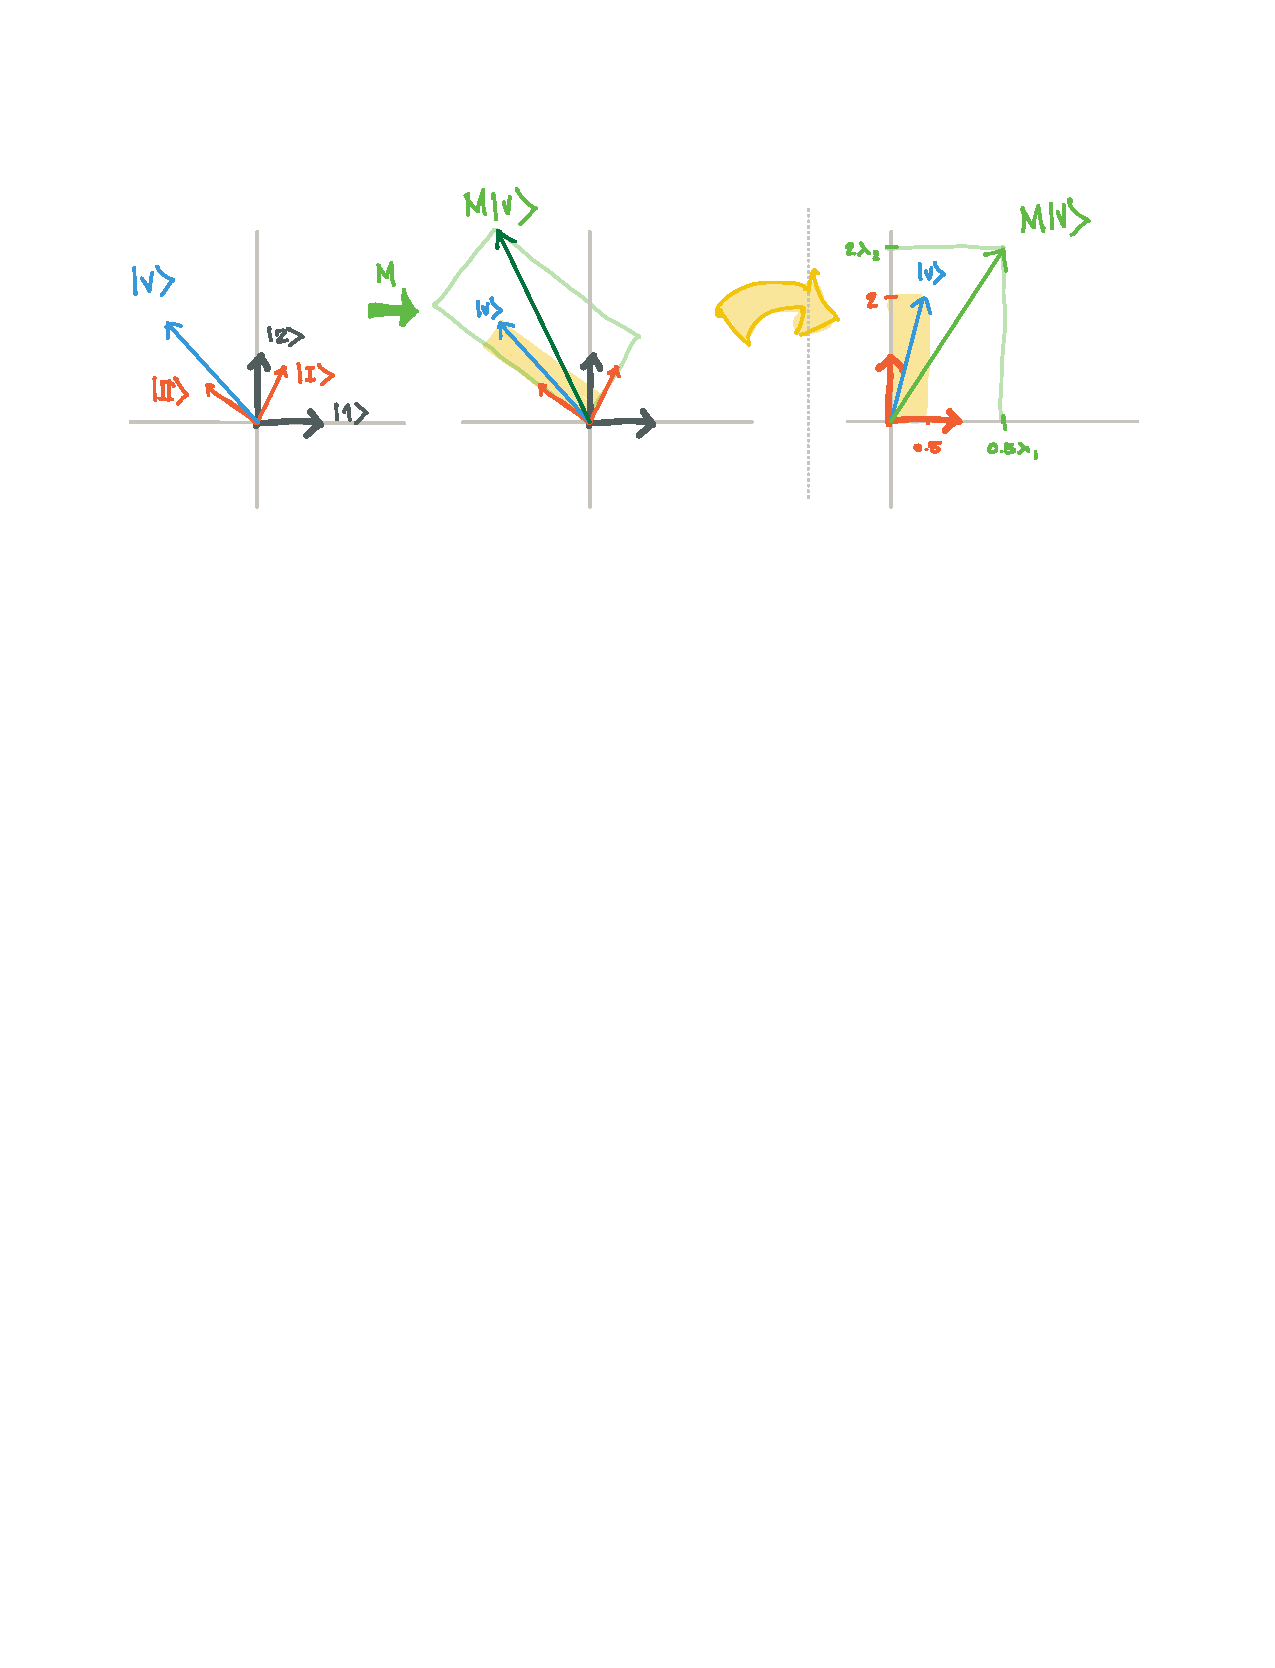
\includegraphics[width=.8\textwidth]{figures/eigen_transform.pdf}
    \caption{Standard basis (black) and eigenbasis (red) vectors and the vector $\ket{v}$ (blue) in \eqref{eq:eigen:example:v}. Under a transformation $M$, the vector is mapped to $M\ket{v}$ (green) which is a rescaling of the components of $\ket{v}$ along the eigenbasis directions (shown as a green box). Right: the transformation as seen by an eigen-observer's frame.}
    \label{fig:eigentransform}
\end{figure}

Passing to the eigenbasis gives a clear understanding of what a Hermitian linear transformation does. We sketch this in Figs.~\ref{fig:eigentransform} and \ref{fig:eigenbal}. For that example, we consider a matrix $M$ with eigenvectors $\ket{{\text{I},\text{II}}}$ and corresponding eigenvalues $\lambda_{\text{I},\text{II}}$:
\begin{align}
    M &= \begin{pmatrix}
        2 & 1 \\
        1 & 3
    \end{pmatrix}
    &
    \lambda_{\text{I},\text{II}} &\approx 3.6,\; 1.4 \ .
    &
    \ket{\text{I}},\ket{\text{II}}&\approx
    \begin{pmatrix}
        0.5 \\ 0.9
    \end{pmatrix},
    \;
    \begin{pmatrix}
        -0.9 \\ \pp 0.5
    \end{pmatrix} \ .
\end{align}
Figure~\ref{fig:eigentransform} shows a vector 
\begin{align}
    \ket{v} = 0.5\ket{\text{I}} + 2\ket{\text{II}} \approx
    -1.4\ket{1} + 1.5 \ket{2} 
    \label{eq:eigen:example:v}
\end{align}
under the transformation $M$,
\begin{align}
    M\ket{v} = 0.5\lambda_\text{I}\ket{\text{I}} + 2 \lambda_\text{II}\ket{\text{II}} \approx
    -1.4\ket{1} + 3 \ket{2} \ .
    \label{eq:eigen:example:Mv}
\end{align}
What we see is that in the eigenbasis, $M$ simply \emph{rescales} the components of $\ket{v}$ along the eigenbasis directions. 


\begin{figure}[tb]
    \centering
    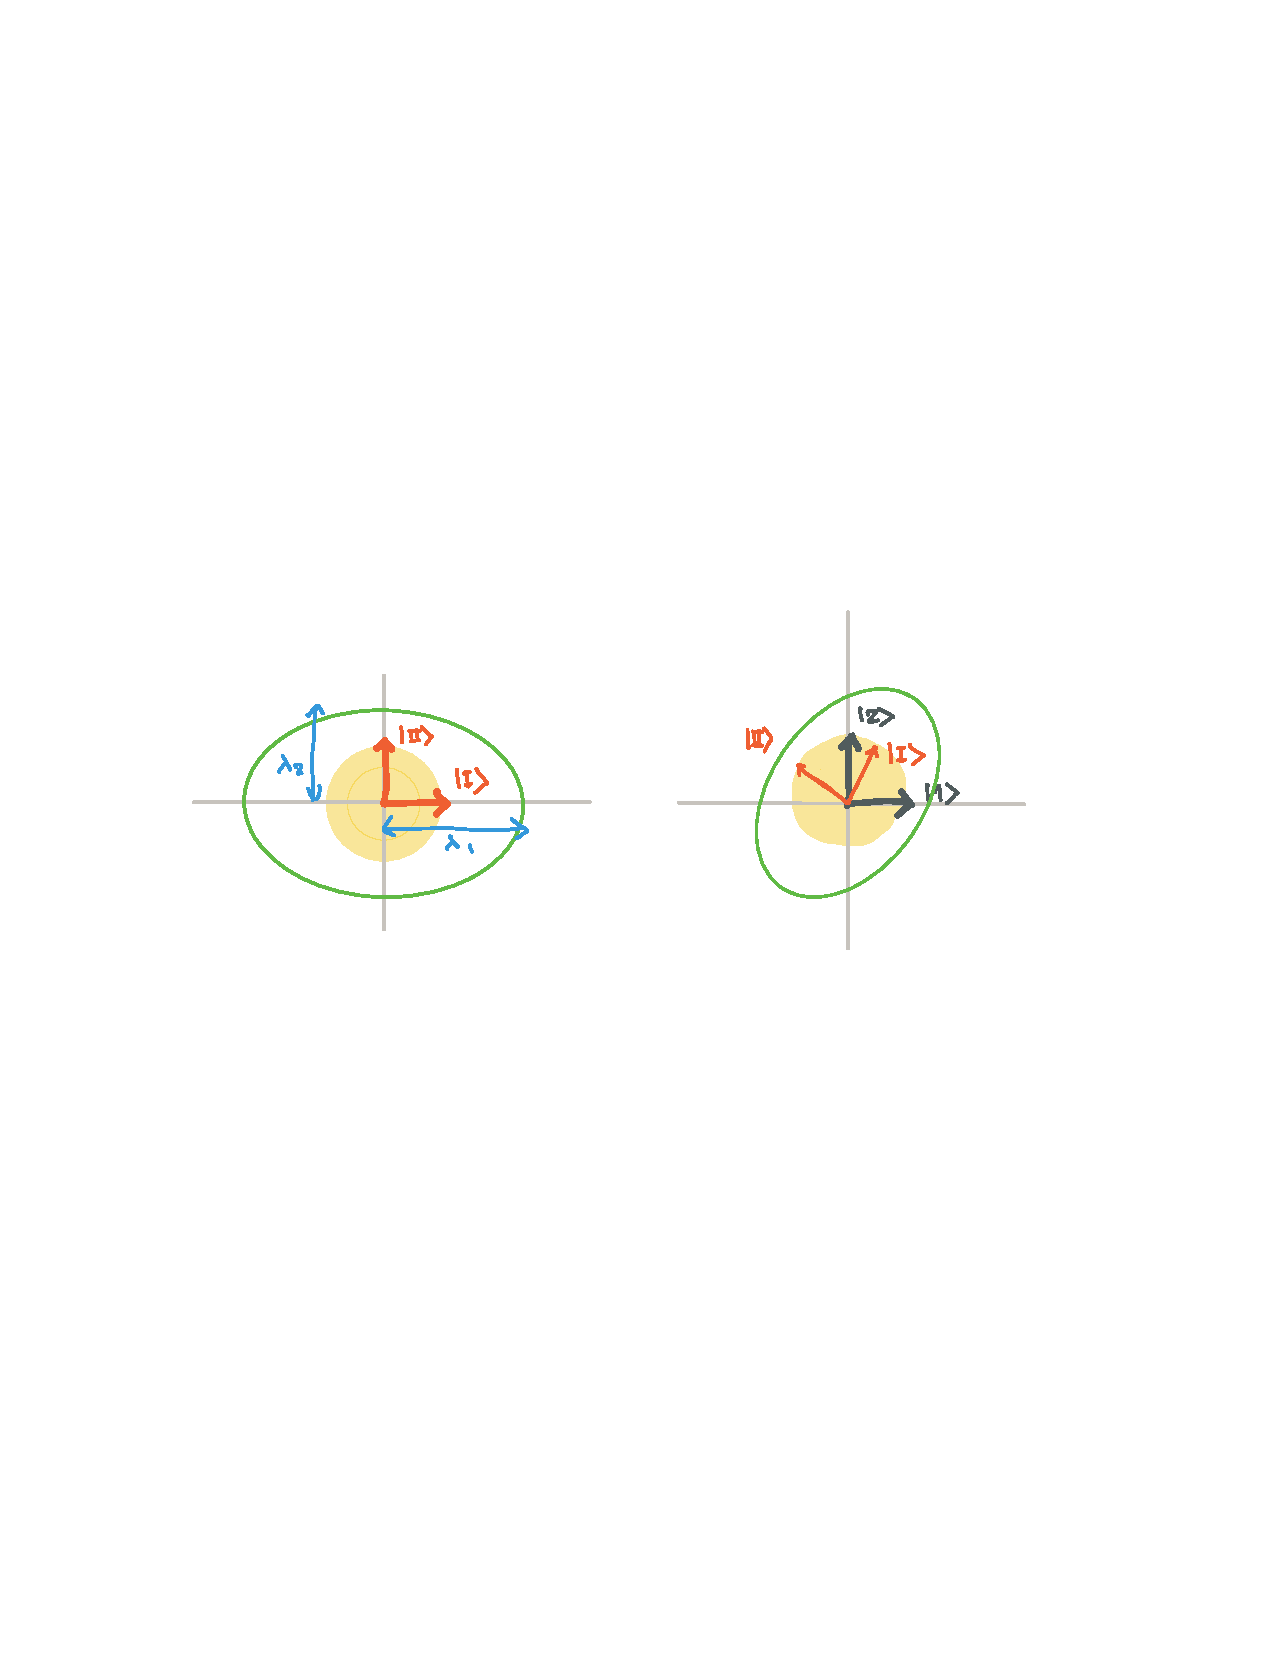
\includegraphics[width=.8\textwidth]{figures/eigen_ball.pdf}
    \caption{Eigenbasis directions are shown in red. The surface of the yellow ball represents all vectors of unit length. The green ellipse represents the deformation of this surface by acting on each of those vectors by $M$. We see that the eigenbasis components of these vectors are simply rescaled by the eigenvalues of $M$. Right: Same figure, but drawn relative to the standard basis.}
    \label{fig:eigenbal}
\end{figure}

Figure~\ref{fig:eigentransform} shows a unit ball in the eigenbasis and how it is deformed under $M$. The surface of the ball should be understood as endpoints of a set of possible vectors. Under $M$, this surface is deformed to the green ellipse. In the standard basis, this ellipse is skewed by the rotation between the two bases. 


\begin{bigidea}
Let us revisit our pantheon of nice matrices that we presented in Section~\ref{sec:hierarchy:of:transformations}. The gold medal (proportional to identity) matrices were too simple: they behave like numbers. The silver medal matrices are those matrices that are already in an eigenbasis. The bronze medal matrices are the kinds of matrices that you will most likely have to deal with ``in the field.'' These matrices that are diagonalizable by a rotation, but that are not yet in an eigenbasis. The meaning of these kinds of transformation is simply a rescaling along a set of orthogonal axes---with independent rescaling along each direction. 

You can also start to imagine what a generic `trash' matrix does. If the matrix is non-invertible, it is some sort of projection. It throws out information. If the matrix is invertible but not diagonalizable by a rotation, then it means that it is not simply rescaling along a set of orthogonal directions. For example, it may be a rescaling along a set of non-orthogonal directions. 
\end{bigidea}

\begin{exercise}
Trash matrices that are invertible but not diagonalizable by a rotation can usually still be diagonalized. You can look up the procedure, it is called a singular value decomposition. The matrix can be made diagonal not by a rotation $M_\text{trash}\to RM_\text{trash}R^\dag$, but by ``half rotation'' by two different rotation matrices: $M_\text{trash} \to SM_\text{trash} R^\dag,$ where $S \neq R$. One way to find these matrices is to diagonalize the Hermitian matrices $N=M^\dag M$ and $L = M M^\dag$. Show that $N$ and $M$ are indeed Hermitian and that they are diagonalized by $S$ and $R$ .
\end{exercise}






\section{Degenerate Eigenvalues}
% commutators
% start with trivial example, diagonal 

Sometimes a matrix will have degenerate eigenvalues. This means that $\lambda_i = \lambda_{i+1}$ for some pair of eigenvalues. We continue to assume that the eigenvalues are all non-zero, as required for invertible (nice!) matrices.  Degenerate eigenvalues can lead to some curiosities when applying the `standard procedure' above. 

\subsection*{Diagonal Matrix}

Let us start with the simplest case where we have a diagonal $3\times 3$ matrix, $\hat M$, with a pair of degenerate eigenvalues\footnote{That means that the eigenvalues are the same, not that they are somehow immoral.}:
\begin{align} 
    \hat M &= 
    \begin{pmatrix}
        \lambda_1 & & \\
        & \lambda_\text{d} & \\
        & & \lambda_\text{d} \ .
    \end{pmatrix}
    &
    \lambda_\text{d}  \neq \lambda_1\ .
    \label{eq:degenerate:eigenvalue:diagonal}
\end{align}
It should be obvious that the eigenvalues are $\lambda_{1,\text{d}}$ and that we can choose eigenvectors $\ket{1}$, $\ket{2}$, $\ket{3}$. That is: the standard basis is an eigenbasis. After all, that's what it means for a matrix to be diagonal in a basis. 

Just for the sake of argument, let us try to `derive' the eigenvectors. The first eigenvalue equation is
\begin{align}
    \begin{pmatrix}
        \lambda_1 & & \\
        & \lambda_\text{d} & \\
        & & \lambda_\text{d} \ .
    \end{pmatrix}
    \begin{pmatrix}
        x\\y\\z
    \end{pmatrix}
    &= 
    \lambda_1
    \begin{pmatrix}
        x\\y\\z
    \end{pmatrix} \ .
\end{align}
We can solve this to find that $x$ can be anything and $y=z=0$ because $\lambda_1\neq \lambda_\text{d}$. The normalized choice is that the first eigenvector is $\ket{1}$. Curiously, second and third eigenvalue equations are the same:
\begin{align}
    \begin{pmatrix}
        \lambda_1 & & \\
        & \lambda_\text{d} & \\
        & & \lambda_\text{d} \ .
    \end{pmatrix}
    \begin{pmatrix}
        x\\y\\z
    \end{pmatrix}
    &= 
    \lambda_\text{d}
    \begin{pmatrix}
        x\\y\\z
    \end{pmatrix} \ .
    \label{eq:eigenvalue:degenerate}
\end{align}
We can see that $x=0$, but there appears to be no constraints on $y$ or $z$ other than that they eigenvectors are normalized. How are we supposed to pick them? Let us take stock of the situation: We know that the standard basis vectors $\ket{2}$ and $\ket{3}$ work as eigenvalues. Why doesn't the eigenvalue equation \eqref{eq:eigenvalue:degenerate} just tell us that? If we stuck in \emph{any} values for $y$ and $z$, then it appears that \eqref{eq:eigenvalue:degenerate} is still satisfied! Curious!

The degeneracy of the second and third eigenvalues has created a degeneracy in how we define our eigenvectors. One way of thinking about this is that the lower $2\times 2$ block of $\hat M$ is a $2\times 2$ matrix proportional to the identity. This means if we did a rotation on that block, it does not change:
\begin{align}
    \bar R \hat M R^\dag &= \hat M
    &
    \bar R&=
    \begin{pmatrix}
        1 & & \\
        & \cos\theta & -\sin\theta \\
        & \sin\theta & \pp \cos\theta
     \end{pmatrix} \ .
     \label{eq:rot:lower:2}
\end{align}
In the same way, it does not matter how we orient our $\ket{2}$ and $\ket{3}$ basis vectors in this plane as long as (1) they are orthogonal to each other and (2) they are normalized. Any rotation of these two vectors into each other is not only a legitimate basis (which is always true), it is still a legitimate eigenbasis of $\hat M$, see Fig.~\ref{fig:det:eig:rot}:
\begin{align}
    \ket{2'} &= \cos\theta \ket{2} -\sin\theta \ket{3}
    &
    \ket{3'} &= \sin\theta \ket{2} +\cos\theta \ket{3} \ .
\end{align}
% 
\begin{figure}[tb]
    \centering
    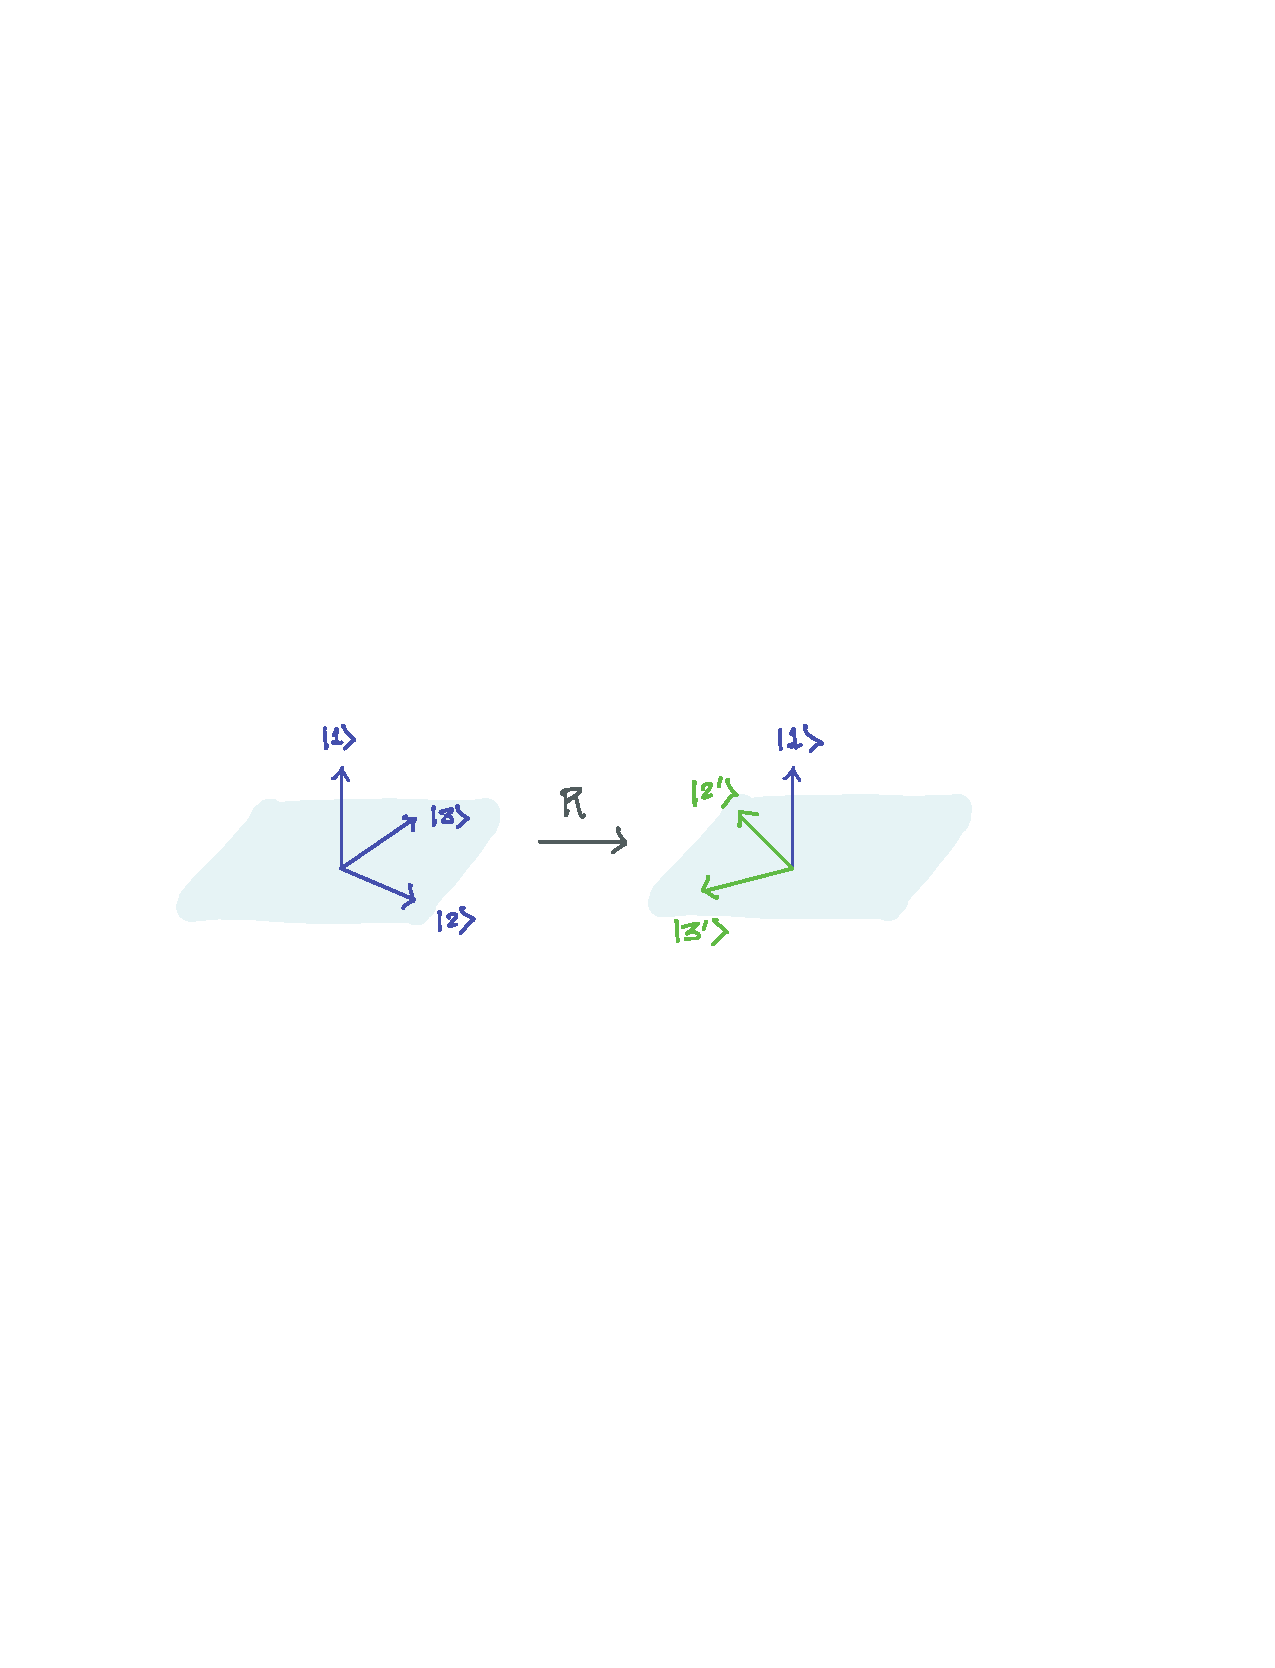
\includegraphics[width=.8\textwidth]{figures/deg_eig_rot.pdf}
    \caption{Example of a rotation of a subspace while leaving one direction in the full space unchanged.}
    \label{fig:det:eig:rot}
\end{figure}
% 

\subsection*{Hermitian Matrix}

So far so good. What happens with general Hermitian matrices with degenerate eigenvalues? We can reduce this case to the case of a diagonal matrix and deduce that the degeneracy in the eigenbasis appears in this more general case as well. To start, we remember that any Hermitian matrix $M$ can be written as a rotation of a diagonal matrix, $\hat M$: 
\begin{align}
    M = R \hat M R^\dag \ .
\end{align}
Suppose that $M$ has eigenvalues, $\lambda_1$ and $\lambda_\text{d}$, where the latter eigenvalue has ``multiplicity two.'' This is our fancy way of saying that there are two eigenvalues that are $\lambda_\text{d}$. This just means that $\hat M$ takes the form in \eqref{eq:degenerate:eigenvalue:diagonal}. 

From Section~\ref{sec:rotation:to:eigenbasis}, we know that the eigenvectors are 
\begin{align}
    \ket{\text{A}} &= (R^\dag)\aij{i}{A}\ket{i} \ .
    &
    A = \{\text{I, II, III}\} \ .
    \label{eq:eigenvectors:from:rotation:review}
\end{align}
\begin{exercise}
Verify \eqref{eq:eigenvectors:from:rotation:review}. One way is to folow the method in Section~\ref{sec:rotation:to:eigenbasis}. Another way is to use the fact that $M = R\hat{M}R^\dag$ and to notice that $\hat M$ acts on the eigenbasis. At any rate, make sure you are comfortable with this step. 
\end{exercise}
In the eigenbasis, we know that there is a degeneracy where we can rotate by $\bar R$ in \eqref{eq:rot:lower:2}. That means:
\begin{align}
    M = R \bar R\hat M \bar R^\dag R^\dag \ .
\end{align}
But we see that $R'= R\bar{R}$ is simply a rotation from the eigenbasis to the standard basis. Alternatively, $(R\bar R)^\dag = \bar R^\dag R^\dag$, is the rotation from the standard basis to \emph{an} eigenbasis. We have used the rule for the Hermitian conjugate of a product of matrices, \eqref{eq:adjoint:of:product}. 

We have discovered that both $R^\dag$ and $R'^\dag$ are rotations from the standard basis to valid eigenbases. This means that for any lower $2\times 2$ rotation $\hat R$, we still have an eigenbasis with the same eigenvalues. 



\begin{bigidea}
When there is a degeneracy in the eigenvalues of a matrix, there is a degeneracy in the definition of the corresponding eigenvectors. A better word to use is symmetry: if two eigenvalues are the same, then there is a symmetry that allows us to rotate the corresponding eigenvectors between themselves while preserving the eigenbasis.
\end{bigidea}

\subsection*{Lifting the Degeneracy}

It is often the case that when we have a degenerate eigenvalue, there is a small effect that distinguishes the two eigenvalues. In fact, you may already know examples of this in a different guise: the fine structure of hydrogen. To good approximation, the hydrogen atom's three lowest energy states are a lowest-energy \acro{1S} state and two excited \acro{2P} states. The energies of these states are eigenvalues of a Hamiltonian (``energy matrix''). The two \acro{2P} states correspond to electrons with opposite spins. However, the orbital angular momentum of the electrons creates a little magnetic field that causes one of these degenerate `eigenstates' to have a little more energy and the other to have a little less energy. 

Let us see this in action, albeit for a simpler example. Suppose that in addition to the matrix $\hat M$, you have another matrix, $\hat N$ that \emph{also} is diagonal and \emph{also} is degenerate. (This latter features is not necessary, but helps illustrate our point nicely.) 
\begin{align} 
    \hat N &= 
    \begin{pmatrix}
        \rho_\text{d} & & \\
        & \rho_\text{d} & \\
        & & \rho_3 \ .
    \end{pmatrix}
    &
    \rho_\text{d}  \neq \rho_3\ .
    \label{eq:degenerate:eigenvalue:diagonal:too} 
\end{align}
Observe that the degeneracy in $\hat N$ is in the upper two basis vectors, while the degeneracy in $\hat M$ is in the lower two basis vectors. While the eigenbasis of \emph{either} $\hat N$ \emph{or} $\hat M$ has some freedom to be rotated, there is only \emph{one} eigenbasis that simultaneously leaves $\hat N$ and $\hat M$ diagonal.
\begin{exercise}
Show that the rotation \eqref{eq:rot:lower:2} that represents the degeneracy in $\hat M$ will turn $\hat N$ into a non-diagonal (but Hermitian) matrix. Argue that conversely, the rotation that represents the degeneracy in $\hat N$ sill render $\hat M$ non-diagonal (but Hermitian).
\end{exercise}

If we happen to have these two matrices, then it should be obvious that there is a \emph{best} basis in which we render both of them diagonal. This basis is unique. In fact, because $\hat M$ and $\hat N$ are diagonal in the standard basis, then it is \emph{only} in the standard basis that these two matrices are simultaneously diagonal. Let that sink in: there is no longer any degeneracy in what the eigenvectors are or what their eigenvalues are. They are the following:
\begin{enumerate}
    \item $\ket{1}$ that has eigenvalue $\lambda_1$ under $\hat M$ and $\rho_\text{d}$ under $\hat N$
    \item $\ket{2}$ that has eigenvalue $\lambda_\text{d}$ under $\hat M$ and $\rho_\text{d}$ under $\hat N$
    $\ket{3}$ that has eigenvalue $\lambda_\text{d}$ under $\hat M$ and $\rho_\text{3}$ under $\hat N$ \ .
\end{enumerate}
In fact, we can use the eigenvalues to \emph{label} our eigenvectors:
\begin{align}
    \ket{1} &\equiv \ket{\lambda_1,\rho_\text{d}}
    &
    \ket{2} &\equiv \ket{\lambda_\text{d},\rho_\text{d}}
    &
    \ket{3} &\equiv \ket{\lambda_\text{d},\rho_3} \ .
\end{align}
Thus, for example, $M\ket{\lambda_\text{d},\rho_\text{d}} = \lambda_\text{d}\ket{\lambda_\text{d},\rho_\text{d}}$ or $N\ket{\lambda_\text{d},\rho_3} = \rho_3\ket{\lambda_\text{d},\rho_3}$.
In physics, you will find `kets' with lists of eigenvalues. These simply mean that you are in a system that has many matrices that are simultaneously diagonal. The eigenvectors of that system are being labelled by the simultaneous eigenvalues with respect to these matrices. 

\begin{example}
When we give the electron states in the hydrogen atom funny names, those funny names are precisely labelling the eigenvalues of simultaneously diagonalizable matrices.
\end{example}


\subsection*{Diagonalize all the matrices?}
% commutator

The procedure so far seems to reduce to the following observation: everything is good in an eigenbasis. Why don't we just diagonalize \emph{all the matrices} and work in some mega eigenbasis? Maybe we never have to worry about degenerate eigenvalues because there will always be enough diagonal matrices---like $M$ and $N$ in the previous subsection---to lift all the degeneracies and define a unique eigenbasis.

This is not generally possible. The reason is that the rotation that diagonalizes one matrix is, in general, not the rotation that diagonalizes another. 

\begin{exercise}\label{ex:spin:1:2:Sz:Sx}
Here's a real-world example from quantum mechanics. Consider the spin of an electron. The spin can be measured along any axis. Let us consider the $z$- axis and the $x$-axis. The spin measurement is encoded in the eigenvalues of the following spin matrices:
\begin{align}
    \hat S_z &= \frac{\hbar}{2}
    \begin{pmatrix}
    1 & \\ 
    & -1     
    \end{pmatrix}
    &
    \hat S_x &= \frac{\hbar}{2}
    \begin{pmatrix}
     & 1\\ 
    1 &    
    \end{pmatrix} \ .
\end{align}
Please check that both of these matrices have eigenvalues $\pm \hbar/2$. The first matrix is already in an eigenbasis, while the second is not. Show that diagonalizing $\hat S_x$ will cause $\hat S_z$ to be not-diagonal.  

\textbf{Comment}: in quantum mechanics, measurements are associated with Hermitian matrices. The eigenvalues of the Hermitian matrix  encodes the possible values that one may measure. Here we see that the spin of the electron is $\pm 1/2$ along some measurement axis. 
\end{exercise}

\begin{exercise}\label{ex:spin:1:2:Sz:Sx:prob}
Vectors in quantum mechanics are possible states of a system. A state that is an eigenvector of a Hermitian matrix is one where there is no uncertainty in the value of a measurement. If a state is a linear combination of eigenstates, $\ket{\psi} = a \ket{\text{I}}+b\ket{\text{II}}$, then the probability of measuring a particular eigenvalue is the squared absolute value of its eigenvector coefficient. That is: given a state $\ket{\text{I}}$, the probability of measuring eigenvalue $\lambda_\text{I}$ is $|a|^2$. 

We assume that the states are always normalized, so $|a|^2 + |b|^2 = 1$. In Example~\ref{ex:spin:1:2:Sz:Sx}, suppose you started with a state $\ket{\psi} = \ket{\lambda_z = +\hbar/2}$. That is, the eigenstate with $\hat S_z$ eigenvalue $\lambda_z = \hbar/2$. Write this in the eigenbasis of $\hat S_x$. Show that the state of \emph{definite} spin in the $z$-direction has \emph{maximally uncertain} spin in the $x$-direction. That means that the probabilities of measuring spin in the $x$-direction to be either $\pm\hbar/2$ is 50\%. 
\end{exercise}


Maybe that's fair enough. If every matrix could be diagonalized then we would never deal with non-diagonal matrices. But now we have a more pressing question. Suppose you have two different Hermitian matrices, $M$ and $N$. You know that they can both be diagonalized, but you do not know if they can be \emph{simultaneously} diagonalized. This is an critical question. There are two possibilities:
\begin{enumerate}
    \item The two matrices can be simultaneously diagonalized. They are different only because they have different eigenvalues. Then there is a rotation $R$ such that 
    \begin{align}
        M &= R \hat M R^\dag
        &
        N &= R \hat N R^\dag \ ,
    \end{align}
    where $\hat M$ and $\hat N$ are diagonal. The rotation $R^\dag$ is the transformation to go from the standard basis to the eigenbasis.
    \item The two matrices cannot be simultaneously diagonalized. They may even have the same eigenvalues (in general they will not), but there is no basis where both $M$ and $N$ are diagonal. In other words:
     \begin{align}
        M &= R \hat M R^\dag
        &
        N &= S \hat N S^\dag 
        &
        S\neq R \ .
    \end{align}
\end{enumerate}
You could simply diagonalize both matrices and see what happens. Unfortunately, as algorithmic as we have made the procedure of diagonalization---that is, finding the eigenvectors---it is still kind of a pain to do this to every single matrix we meet. Is there perhaps an easier way to see whether or not two matrices are simultaneously diagonalizable?

\begin{example}
If you have two diagonal matrices, $\hat M$ and $\hat N$, then the two matrices are obviously simultaneously diagonalizable. However, the multiplication of diagonal matrices reduces to the multiplication of the diagonal elements as numbers. This means that
\begin{align}
    \hat M \hat N &= \hat N \hat M
    &\Rightarrow&&
    \left[\hat M, \hat N\right] &= 0
    \ .
\end{align}
Here we have used the definition of the \textbf{commutator}, $[A,B] = A,B$. We say that two matrices \textbf{commute} if their commutator vanishes. We have shown that diagonal matrices commute.
\end{example}

If you are already in the basis where two matrices are diagonal, then the question is moot. The answer to whether they are simultaneously diagonalizable is solved. The observation that $[\hat M,\hat N] =0 $ for simultaneously diagonalizable matrices holds for any pair of Hermitian matrices. Let us see why. Let us take our diagonal matrices and rotate them by some matrix $R$ to go to any other basis where they are non-diagonal but Hermitian. Then we have matrices
\begin{align}
    M &= R \hat M R^\dag
    &
    N &= R \hat N R^\dag \ .
\end{align}
We can write the diagonal matrices in terms of their rotated form and plug this into the commutator:
\begin{align}
    0=
    \left[ R^\dag M R, R^\dag N R  \right] 
    \\&= 
    R^\dag M R R^\dag N R
    -
    R^\dag N R R^\dag M R
    \\&=
    R^\dag(MN - NM)R
    \\&= R^\dag \left[M,N\right] R \ .
\end{align}
Here we have used $RR^\dag =\one$. We can multiply both sides by $R$ from the left and $R^\dag$ on the right---or we may simply argue that rotating a matrix cannot cause it to vanish---to find that the commutator of the matrices vanishes:
\begin{align}
    \left[M,N\right] = 0 \ .
\end{align}
Critically, this is true in \emph{any} basis, whether or not $M$ and $N$ are diagonal in that basis. Further, you can show that this is true \emph{only} when $M$ and $N$ are simultaneously diagonalizable. 

If $M$ and $N$ are not simultaneously diagonalizable, then we could \emph{try} to massage their commutator into a commutator of diagonal matrices:
\begin{align}
    \left[M,N\right] = 
    \left[R\hat M R^\dag, S\hat N S^\dag\right]
    =
    R \hat M R^\dag S \hat N S^\dag
    -
    S \hat N S^\dag    R \hat M R^\dag  \ .
\end{align}
We see that $R^\dag S$ and $S^\dag R$ do not equal to $\one$ and so we cannot massage this into a form where we get $[\hat M, \hat N]$. 

\begin{bigidea}
Matrices are simultaneously diagonalizable if they all commute with one another, $[M,N] = 0$. When this is the case, there is a single eigenbasis where all the matrices are diagonal. If some of the matrices have degenerate eigenvalues, it is possible that other matrices can lift those degeneracies. In this way, it is convenient to label eigenvectors by their unique combination of eigenvalues with respect to the set of commuting matrices. 

When matrices do not commute, they cannot be simultaneously diagonalized. In quantum mechanics, two observables that do not commute are observables that you cannot simultaneously measure. This is the algebraic manifestation of quantum uncertainty.
\end{bigidea}


\section{Inverting Nice Matrices}
\label{sec:inverting:nice:matrices}
\flip{To do: fix the clunky notation in these sections.}

The power of all of this eigenstuff is that we can solve problems of the following form
\begin{align}
    M \ket{v} = \ket{s} \ ,
    \label{eq:Mv:s}
\end{align}
where we are given a nice matrix $M$ and the output vector $\ket{s}$. We are asked to solve for $\ket{v}$. The solution is obviously $\ket{v} = M\inv \ket{s}$. Because $M$ is `nice,' we know it is invertible---after all, it is a Hermitian matrix with non-zero eigenvalues. For small and simple matrices, you can simply solve $M\inv M = \one$ component-by-component. For moderately difficult matrices you can plug this into a computer. However, we will soon concern ourselves with the problem of \emph{infinite dimensional} vector spaces. In this limit, the problem \eqref{eq:Mv:s} becomes a differential equation 
\begin{align}
    \mathcal O f(x) = s(x) \ ,
    \label{eq:Of:s}
\end{align}
where $\mathcal O$ is a differential operator like $-(d/dx)^2$. The vector $\ket{v}$ is now written as a function $f$ and the discrete component index $i$ of $v^i$ has become a continuous argument $x$ in $f(x)$. You are familiar with these differential equations: they show up all the time in physics. 
\begin{example}
Newton's law of motion is
\begin{align}
    m\frac{d^2}{dt^2} \vec{x}(t) = -\nabla V[x] \ ,
\end{align}
where $V$ is the potential of the force. 
\end{example}
For this infinite-dimensional limit, the best way to solve \eqref{eq:Of:s} is to rotate into a basis of \emph{eigenfunctions} and use the fact that the action of $\mathcal O$ simplifies greatly in this basis.

It is thus instructive to walk through the process of solving \eqref{eq:Mv:s} using a rotation to to the eigenbasis. It may seem silly that we do things this way for a $2\times 2$ matrix, but this example will make it clear how everything works. To this end, let us solve \eqref{eq:Mv:s} with the following values:
\begin{align}
    M &= 
    \begin{pmatrix}
        9 & -\sqrt{3}\\
        -\sqrt{3} & 11
    \end{pmatrix}
    &
    v^i &= 
    \begin{pmatrix}
        x \\ y
    \end{pmatrix}
    &
    s^i &=
    \begin{pmatrix}
        a \\ b
    \end{pmatrix} \ .
\end{align}
We choose explicit numbers for the components of $M$ so that we can write out explicit eigenvalues and derive explicit eigenvectors. We would like to find the components $v^i$ in the standard basis, which we have labelled as $x$ and $y$. For the source, $s^i$, we simply assume some \emph{a priori} known values $a$ and $b$. In fact, our solution will depend linearly on $a$ and $b$ so that we will have solved the problem of inverting this matrix $M$ for \emph{any} source. 


\paragraph{Characteristic equation} First we solve for the eigenvalues of $M$. The characteristic equation is
\begin{align}
    0=\det(M-\lambda \one) &= 
    (9-\lambda)(11-\lambda) - 3
    &
    \lambda_{\text{I},\text{II}}&= 8,12 \ .
\end{align}

\paragraph{Eigenvectors} The eigenvectors come from solving $M\ket{A} = \lambda_A \ket{A}$ for $A=\text{I}, \text{II}$. The general form of this equation is
\begin{align}
    9q - \sqrt{3}s &= \lambda_A q
    &
    -\sqrt{3}q + 11 s &= \lambda_B s \ ,
\end{align}
where the standard basis components of $\ket{A}$ are $s$ and $q$. Of course, only one of these equations is sufficient to specify the relation between the two components of the eigenvector $\ket{A}$: the other is redundant.\footnote{Be sure you are clear \emph{why} the second equation has to be redundant. The eigenvalue equation is true even for $\ket{A}\to \alpha\ket{A}$, so it cannot determine the normalization of the eigenvectors.} This fixes the ``direction'' of the eigenvector. We find that the eigenvectors are proportional to 
\begin{align}
    \ket{\text{I}}
    &\propto 
    \begin{pmatrix}
        \sqrt{3}\\ 1
    \end{pmatrix}
    &
    \ket{\text{II}}
    &\propto 
    \begin{pmatrix}
        1\\ -\sqrt{3}
    \end{pmatrix} \ .
\end{align}
Since this is a two dimensional space, one could have simply used orthogonality to deduce $\ket{\text{II}}$ from $\ket{\text{I}}$. Normalizing the eigenvectors according to $\la A | A\ra = 1$ gives us
\begin{align}
    \ket{\text{I}}
    &=
    \frac{\sqrt{3}}{2} 
    \ket{1}
    + 
    \frac{1}{2}
    \ket{2}
    &
    \ket{\text{II}}
    &=
    \frac{1}{2}
    \ket{1} 
    - 
    \frac{\sqrt{3}}{2}
    \ket{2}
    \ .
    \label{eq:ex:greens:func:eig:in:std}
\end{align}

\paragraph{Rotating to the eigenbasis} Now that we have the components of the eigenbasis in terms of the standard basis, $\la i | A \ra$, we know all of the components of the rotation matrix between the two bases, as we saw in Section~\ref{sec:rotation:to:eigenbasis}. If you're like me, you always get confused about whether these components are the rotation from the standard basis to the eigenbasis, or from the eigenbasis to the standard basis. Do we arrange them as rows or as columns? It is worth taking a moment to sort that out without looking at Section~\ref{sec:rotation:to:eigenbasis}. For the sake of pedagogy, let us do this a bit more tediously but straightforwardly. Let us invert \eqref{eq:ex:greens:func:eig:in:std} to write the standard basis vectors in terms of the eigenbasis vectors.\footnote{This is, of course, a rotation.} By taking appropriate linear combinations, we find that
\begin{align}
    \ket{1}
    &=
    \frac{\sqrt{3}}{2} 
    \ket{\text{I}}
    + 
    \frac{1}{2}
    \ket{\text{II}}
    &
    \ket{2}
    &=
    \frac{1}{2}
    \ket{\text{I}}
    - 
    \frac{\sqrt{3}}{2}
    \ket{\text{II}}
    \ .
    \label{eq:ex:greens:func:std:in:eig}
\end{align}
You might object that \eqref{eq:ex:greens:func:std:in:eig} does not look like much of a rotation. You may recall that this is the form of a rotation with a discrete isometry, \eqref{eq:discrete:isometry:eg}. What has happened is that we have changed the relative orientation\footnote{I say this somewhat colloquially because the term `orientation' has a more formal meaning.} of the basis vectors. Or, in other words, maybe we should have chosen a different overall sign for one of the eigenvectors in \eqref{eq:ex:greens:func:eig:in:std}. No matter! We press forward.

Inserting \eqref{eq:ex:greens:func:std:in:eig} into our expression for $\ket{v}$, we find the components of $\ket{v}$ in the eigenbasis:
\begin{align}
    \ket{v} &=
    x\ket{1} + y\ket{2}
    =
    \frac{1}{2}\left(\sqrt{3}x+y\right)\ket{\text{I}}
    +
    \frac{1}{2}\left(x-\sqrt{3}y\right)\ket{\text{II}}
    \equiv
    x' \ket{\text{I}} + y' \ket{\text{II}} \ .
\end{align}
Similarly, the components of the source $\ket{s}$ are
\begin{align}
    \ket{s} &=
    \frac{1}{2}\left(\sqrt{3}a+b\right)\ket{\text{I}}
    +
    \frac{1}{2}\left(a-\sqrt{3}b\right)\ket{\text{II}}
    \equiv
    a' \ket{\text{I}} + b' \ket{\text{II}} \ .
    \label{eq:eigen:greens:eg:source:components:eig}
\end{align}
The primed variables are the components in the eigenbasis. Now that our kets are written as linear combinations of eigenvectors, the action of $M$ is straightforward. Further, the inverse is simply
\begin{align}
    M\inv = 
    \begin{pmatrix}
        1/\lambda_\text{I} &\\
        & 1/\lambda_\text{II}
    \end{pmatrix} \ .
\end{align}
This means that the equation $M\ket{v}=\ket{s}$ is
\begin{align}
    \begin{pmatrix}
        \lambda_\text{I} & \\
        & \lambda_\text{II}
    \end{pmatrix}
    \begin{pmatrix}
        x' \\ y'
    \end{pmatrix}
    =
    \begin{pmatrix}
        a' \\
        b'
    \end{pmatrix} \ ,
\end{align}
from which we straightforwardly deduce
\begin{align}
    x' &= \frac{a'}{\lambda_\text{I}}
    &
    y' &= \frac{b'}{\lambda_\text{II}} \ .
\end{align}
This formally solves the problem, though we should be courteous and state the result in the standard basis.\footnote{This is similar to the etiquette that you should re-rack your weights in the gym.}

\paragraph{Rotating back to the standard basis} We have already written transformation back to the standard basis, \eqref{eq:ex:greens:func:eig:in:std}. It is straightforward to plug this into our solution in the eigenbasis. For the sake of pedagogy, let us try to write this a a rotation. We find that
\begin{align}
    \frac{1}{2}
    \begin{pmatrix}
        \sqrt{3} & 1\\
        1 & -\sqrt{3}
    \end{pmatrix}
    \begin{pmatrix}
        x \\ y
    \end{pmatrix}
    = 
    \begin{pmatrix}
        x' \\ y'
    \end{pmatrix}
    =
    \begin{pmatrix}
        a'/\lambda_{I}\\
        b'/\lambda_{II}
    \end{pmatrix} \ ,
\end{align}
where we have explicit expression for $a'$ and $b'$ in terms of the original source components $a$ and $b$ in \eqref{eq:eigen:greens:eg:source:components:eig}. We recall that this matrix is not a rotation, but rather a rotation and a discrete isometry. We may simplify the problem by multiplying both sides by the discrete isometry 
\begin{align}
    P = \begin{pmatrix}
        1 & \\
        & - 1
    \end{pmatrix} 
\end{align}
to to ``undo'' the discrete isometry and recover a rotation matrix
\begin{align}
    \frac{1}{2}
    \begin{pmatrix}
        \sqrt{3} & 1\\
        -1 & \sqrt{3}
    \end{pmatrix}
    \begin{pmatrix}
        x \\ y
    \end{pmatrix}
    &=
    \begin{pmatrix}
        \pp a'/\lambda_{I}\\
        -b'/\lambda_{II}
    \end{pmatrix} 
    &
    \begin{pmatrix}
        x \\ y
    \end{pmatrix}
    &=
    \frac{1}{2}
    \begin{pmatrix}
        \sqrt{3} & -1\\
        1 & \sqrt{3}
    \end{pmatrix}
    \begin{pmatrix}
        \pp a'/\lambda_{I}\\
        -b'/\lambda_{II}
    \end{pmatrix} \ ,
\end{align}
On the right-hand side we have used the fact that the inverse of a rotation is simply its transpose. 


\begin{subappendices}
\section{Another proof that diagonal becomes symmetric}
\label{sec:another:proof:diag:is:symmetric}

We present an alternative proof of Theorem~\ref{thm:symmetric:rotates:to:symmetric}. The proof is a little tedious and may be skipped on a first reading.
% 
% \begin{proof}
We use the fact that because $D$ is self-adjoint in the following form:
\begin{align}
    \la Dv, w \ra = \la v, Dw\ra \ .
\end{align}
Now we use the fact that rotations (isometries) $R$ preserve the inner product so that
\begin{align}
    \la RDv, Rw \ra = \la Rv, RDw \ra \ .
\end{align}
In components this is
\begin{align}
    R\aij{i}{j}D\aij{i}{k} \cancel{v^k}\,
    R\aij{\ell}{m} \cancel{w^m}\,
    g_{i\ell}
    =
    R\aij{q}{k} \cancel{v^k}\,
    R\aij{s}{t} D\aij{t}{m} \cancel{w^m}\,
    g_{qs} \ .
\end{align}
We deliberately chose and labels so that the $v^kw^m$ on each side would have the same indices and those factors could be `canceled out.' We may only do this because the above expression is true for any vectors $\ket{v}$ and $\ket{w}$ and so cannot depend on those components. This means that the objects contracting with these vectors on each side must be equivalent component-wise.  We then contract both sides with $(R\inv)\aij{m}{n}(R\inv)\aij{k}{u}$. The reason for this is that we know that the rotation of a matrix $D\aij{i}{j}$ is $R\aij{i}{k}D\aij{i}{\ell}(R\inv)\aij{\ell}{j}\defeq M$.
\begin{align}
    g_{\ell i} R\aij{i}{j} D\aij{j}{k}\delta^\ell_n
    (R\inv)\aij{k}{u}
    &=
    g_{sq}\delta^q_u R\aij{s}{t} D\aij{t}{m}
    (R\inv)\aij{m}{n}
    \\
    g_{ni} M\aij{i}{u}
    &=
    g_{su} M\aij{s}{n} \ .
\end{align}
We now seek to show that $M$, the rotation of $D$ into another basis\sidenote{Or rather: $M\aij{i}{j}$ are the components of $D$ in a basis \emph{other} than the one where it is diagonal.} is symmetric. Indeed, if we look at the equation above, we may simply lower indices with the metric factors and write out
\begin{align}
    M_{nu} = M_{un} \ ,
\end{align}
which effectively proves our assertion. However, matrices have their first index raised an their second index lowered. So we can multiply both sides by $g^{ur}$ to write
\begin{align}
    g_{ni}M\aij{i}{u}g^{ur} &= M\aij{r}{n} \ .
\end{align}
We recognize the adjoint, \eqref{eq:adjoint:def}, so that $(M^\dag)\aij{r}{n} = M\aij{r}{n}$. This indeed tells us that the rotation of a self-adjoint matrix is self-adjoint. \flip{Is this what we wanted? Since diagonal matrices are self-adjoint, then their rotations are self-adjoint. Then we just have to explain---matthews and walker, theorem 4.7 }

\end{subappendices}
